\section{The LUX Detector} \label{LUXChap} %Talk about self shield in this section
The Large Underground Xenon detector (LUX) is a dual phase time projection chamber located at the Sanford Underground Research Facility in South Dakota.  The detector is a cylindrical structure that uses 370 kg of liquid xenon as a target medium.   The commercially bought xenon was distilled to $\sim$1 ppm (g/g) of air by the manufacturer before undergoing a krypton removal campaign to lower residual krypton levels to less than 5 parts per trillion (g/g). 

Particle interactions in the liquid xenon produce ionized and excited xenon atoms.    The excited xenon atoms form exciton molecules with ground state atoms, subsequently producing scintillation light at 178 nm when the molecules disassociate.  This scintillation light is referred to as the S1 signal.  Some of the electrons released in the ionization process recombine with the xenon ions, forming additional xenon excitons and S1 light, while the rest drift to the liquid surface by an applied electric field.   Electrons which penetrate the liquid surface are accelerated through the gas above the liquid xenon by a stronger electric field, producing electroluminescent light which is referred to as the S2 signal. This process will be discussed in depth in section~\ref{RecombSec} .

Two arrays of 61 PMTs each are used to measure both the S1 and S2 light in the detector.  The light response of each PMT in the top array is used to reconstruct the XY position of recoil events based on the spatial pattern of the S2 signal, and the time difference between the S1 and S2 signal is used to reconstruct the depth of the recoil events via the known drift velocity of electrons in liquid xenon.  In this way, the LUX detector has three dimensional position reconstruction which can be used to define a low-background fiducial volume in the center of the detector.  

 \begin{figure} 
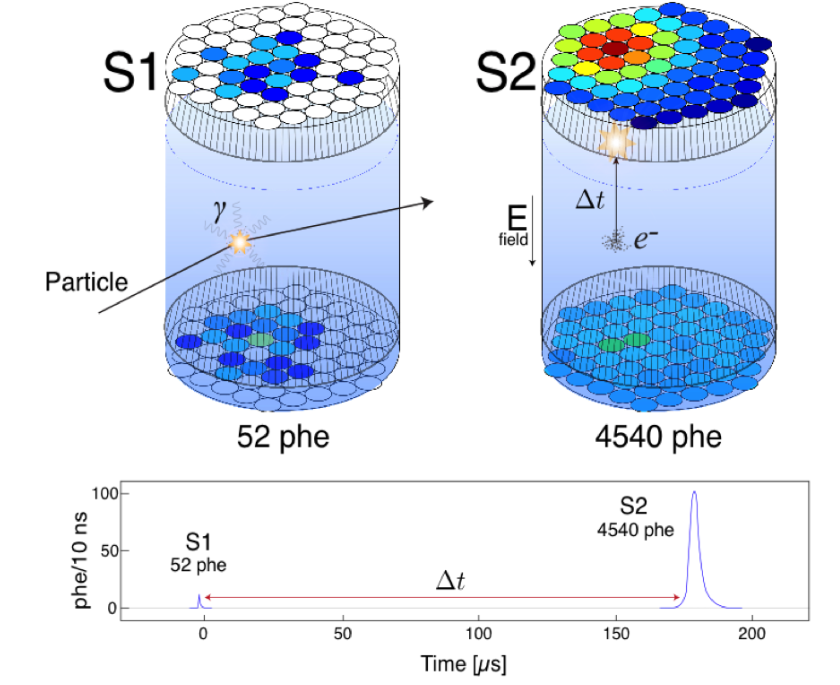
\includegraphics[scale=.5]{LUXevent.png} 
\captionof{figure}{A depiction of a particle event in LUX. The response of the top PMT array to the S2 light is used for xy position reconstruction, while the timing between the S1 and S2 signals is used for the depth measurement.}
\label{LUXevent}
\end{figure}

The center of the LUX detector is an extremely low background environment due to the strong self shielding properties of liquid xenon and the lack of naturally occurring xenon radioisotopes.  Low energy external backgrounds ($<$50 keV) can only travel a few millimeters into the liquid xenon volume, while higher energy gamma rays ($\sim$MeV range) will produce easily identifiable multiscatter events due to their mean free path of a few centimeters.  Residual background events which appear in the fiducial volume are reduced by over 99\% by using the ratio of the S1 and S2 signal as a form of nuclear recoil discrimination.  Discrimination techniques in the LUX detector will be discussed more in section~\ref{DiscrimSec}.  In this section, we will  discuss the detector internals, external support system, and the DAQ electronics used to read out the PMT signal.  

 \begin{figure} 
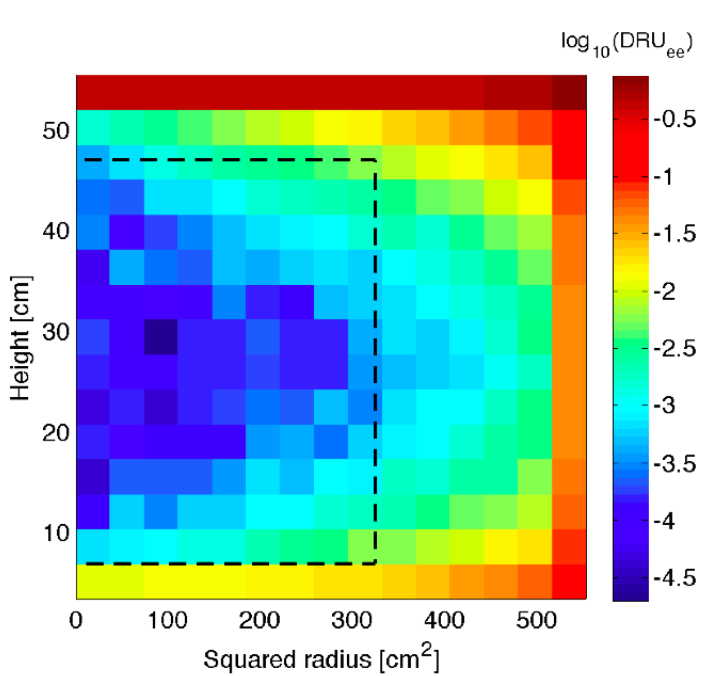
\includegraphics[scale=.5]{GammaBackgrounds.png} 
\captionof{figure}{Simulated gamma ray backgrounds in the LUX detector after removing multiscatter events. The black dashed lines indicate the fiducial volume used in the first LUX WIMP search results.}
\label{GammaBackgrounds}
\end{figure}

\newpage

\subsection{Detector Internals}
\subsubsection{Cryostat} %(Show figure 5 from http://arxiv.org/pdf/1211.3788v2.pdf).


A cross section of the LUX cryostat and detector internals is shown in figure~\ref{LuxCross}.  An outer titanium cryostat is used to maintain a thermally insulating vacuum around the detector.  An inner cryostat which houses the liquid xenon and detector internals is attached to the roof of the outer cryostat via three plastic hangers.  Instrumentation cables and gas circulation plumbing are fed through flexible conduits at the top of the detector.  

 \begin{figure} 
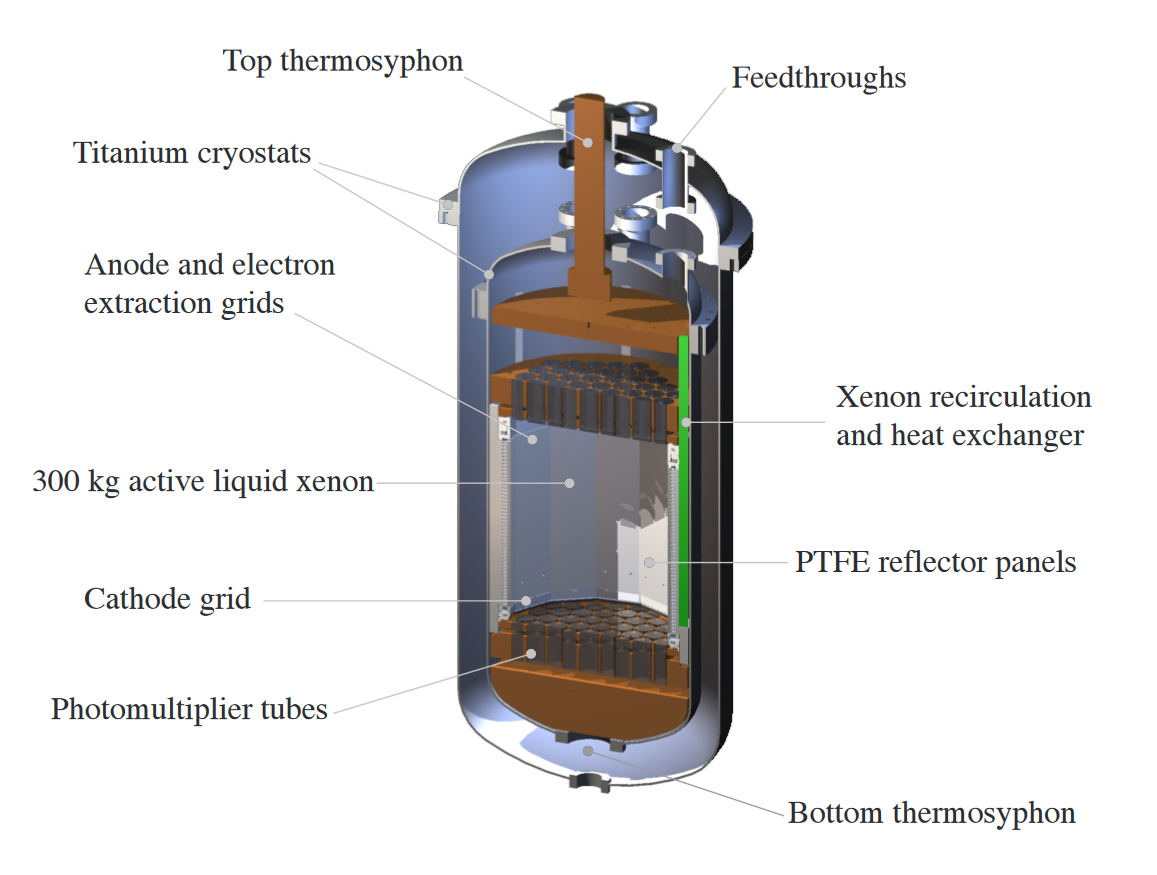
\includegraphics[scale=.45]{LuxCryostat.png} 
\captionof{figure}{Cross section of the LUX cryostats and internal detector components~\cite{LuxDetector}.}
\label{LuxCross}
\end{figure}

	
\subsubsection{PMT Arrays, PTFE Structure, and Field Cage}
Figure \ref{LuxFieldCage} depicts the inside of the inner cryostat, where a 5 cm thick copper block with a diameter of 55 cm is mounted directly on to the flange.  This copper serves as a radiation shield and a temperature controller during detector operations. A similar copper structure is attached to the bottom of the inner cryostat and is used to displace xenon from the inactive volume in addition to performing the functions of the top radiation shield.  

Two PMT arrays collect light from the S1 and S2 signals in the detector.  Each array contains 61 Hamamatsu R8778 PMTs which observe the active volume.  These PMTs were designed for operation in liquid xenon, with a typical quantum efficiency of 33\% at the 178 nm wavelength of liquid xenon scintillation.  The top PMT array is housed in a copper structure which is hung 15 cm below the upper radiation shield by six titanium straps.  Reflective polytetrafluoroethylene (PTFE)   trifoils cover the inner face of the copper housing to increase light collection efficiency in the detector.  A similar structure is placed at the bottom of the detector to house the bottom PMT array. 

Twelve PTFE panels hang from the top PMT support and are attached to the bottom PMT support.  These panels increase the light collection efficiency of the detector, and serve as the support structure for the field cage in the detector.  The electric field is defined by five wire grids.  Each grid is made of stainless streel wires and are 88-99\% transparent at a normal angle of incidence.  Stainless steel is known to be 57\% reflective at the xenon scintillation wavelength, further minimizing the optical footprint of the wire grids.

The top grid is located 2 cm below the top PMT array.  A stainless steel ring is used to string 50 micron diameter stainless steel wires spaced with a pitch of 1 cm.  The voltage on the top grid allows the electric field at the photocathodes of the top PMTs to be zeroed.  The anode is placed 4 cm below the top grid.  It is similar in design to the top grid, but uses 30 micro wires with 0.5 mm spacing. The gate grid, which uses 50 micron stainless steel wires with a pitch of 5 mm, is placed 1 cm below the anode grid. The position of the gate grid places it about 5 mm below the liquid xenon surface.   These two grids work in tandem to produce a strong extraction field (5-6 kV/cm) that pulls charge out of the liquid xenon and into the gas, producing the S2 signal. The cathode grid is placed about 49.5 cm below the liquid surface. This grid uses 260 micron diameter stainless steel wires with a pitch of 5 mm, and works in tandem with the anode grid to produce an electric field which drifts charge from a particle interaction to the liquid surface.  The bottom grid is the last of the five wire grids.  It is located 4 cm below the cathode grid and 2 cm above the bottom PMT support, and uses 206 micron diameter stainless steel wires with a pitch of 1 cm.  The bottom grid serves the similar purpose as the top grid – it is used to zero the field at the photocathodes of the bottom PMT arrays.

Fourty-eight copper field rings are spaced 1 cm apart inside of the PTFE panels to shape the drift field. These rings have thickness of 3.2 mm and a width of 12.7 mm.  The spacing and thickness of the rings were chosen to shield the active region from the electric field produced by the cathode high voltage cable.  The voltage of the field rings is set by a resistor chain that runs between the gate and the cathode grids.  A pair of  0.875 G$\Omega$ resistors connect the top field ring to the gate grid, while a pair of 1.25 G$\Omega$ resistors connect the bottom field ring to the cathode grid.  A pair of 1 G$\Omega$ resistors is used to connect each adjacent field ring.


 \begin{figure} [!h]
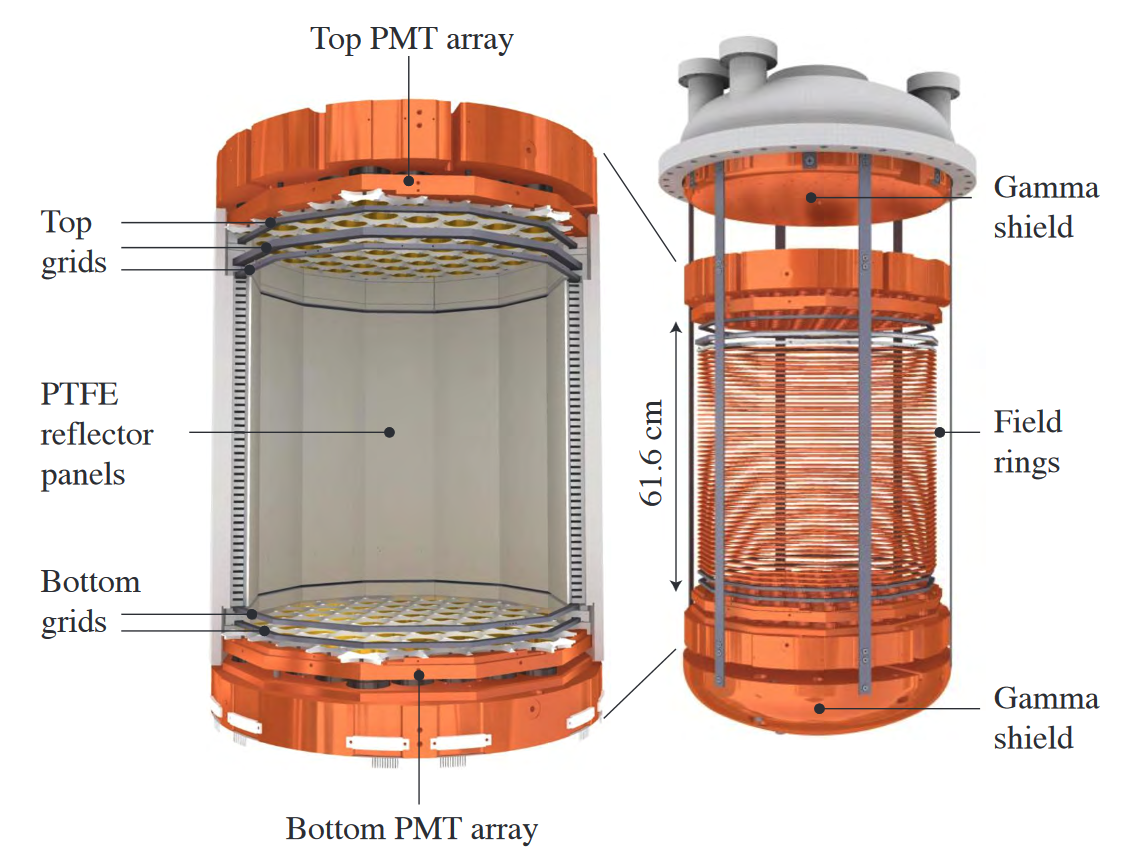
\includegraphics[scale=.45]{LuxFieldCage.png} 
\captionof{figure}{Depiction of the LUX PMT supports, PTFE panels, and field cage~\cite{LuxDetector}.}
\label{LuxFieldCage}
\end{figure}


\subsubsection{Cryogenics}

A thermosyphon system is used to cool the detector internals to liquid xenon temperatures  ($\sim$175K) during operation. A thermosyphon is a sealed tube filled with a variable amount of gaseous nitrogen (N$_2$).  A condenser which is immersed in a bath of liquid nitrogen is placed at the top of the thermosyphon.  As the nitrogen in the thermosyphon tube condenses, gravity causes it to trickle down stainless steel plumbing to copper heat exchangers that are attached to various points in the inner cryostat.  The condensed nitrogen evaporates when it hits the copper heat exchanger, removing heat from the detector.  The evaporated nitrogen rises back up the stainless steel plumbing where it is once again condensed by the liquid nitrogen bath.  In this way, the thermosyphons act in a continuous loop, transferring heat from the detector to the liquid nitrogen bath which the condenser is immersed in.

Two thermosyphons are attached to the copper radiation shields at the top and bottom of the inner cryostat and are used as the driving force to cool the detector from room temperature to 175K. Two more thermosyphons are attached to copper shielding around the inner cryostat and are used to prevent any thermal gradients from building in the detector.  Each copper evaporator is fitted with a 50 W heater and a thermometer for fine temperature control.  Larger 750 W heaters are attached to the two primary thermosyphons to aid in detector warm up during liquid xenon recovery.

\subsubsection{Instrumentation}

The LUX detectors is fitted with numerous instruments that help monitor and stabilize the conditions within the cryostat. Forty 100 $\Omega$ thin film platinum resistance temperature detectors (RTDs) are used to monitor the temperature inside the inner cryostat. These instruments help prevent the formation of thermal gradients which could warp the detector internals.  An additional 23 RTDs monitor the temperature inside the outer vacuum space, providing a means to detect leaks from the inner cryostat or outer atmosphere to the insulating vacuum space. Calibration of the RTD readouts was performed prior to installation, as well as in situ at room temperature, with an accuracy of 170 mK for each RTD.  Advantech Adam 6015 modules feed the output voltage of the RTDs to a slow control database, where multiple users can monitor the values and set automated alarms to notify operators of any temperature fluctuations in the detector.  

A variety of pressure sensors are used throughout the detector.  Sensor models include Ashcroft AST4900 sensors, InstruTech Hornet ion and convection gauge, Swagelok PGU-50-PC100-L4FSF manual pressure gauges, and a Setra model 759 capacitance manometer.  These instruments monitor the stability of the inner cryostat, the quality of the outer vacuum, and the pressure in various locations of the gas circulation system.  As with the RTDs mentioned above, all of the digital pressure gauges are read out to the slow control database where alarms can be set to notify users of potential leaks in the circulation system or out of control warming and cooling effects in the detector.

Six parallel wire sensors monitor the liquid level in the inner cryostat, the weir, dual-phase heat exchanger, and the liquid return line.   The latter detector components mentioned here will be discussed in section~\ref{GasSystem}.  The capacitance of each wire pair depends on the length of wire submerged in the liquid, allowing the overall height of the liquid to be determined.  Additionally, three parallel plate sensors are placed 120 degrees apart between the gate and anode grids.  These sensors ensure the liquid surface is uniform and without any tilt.    


\subsection{External Support Systems}

\subsubsection{Gas Circulation and Purification System} \label{GasSystem}
The xenon used in the LUX detector must be largely free of electronegative and molecular impurities that could attenuate charge and light from particle interactions.  To achieve this goal, LUX circulates the detector’s xenon through a gas system which includes a heated zirconium getter made by SAES.  The getter removes nearly all non-nobel gas impurities with an efficiency of 99.9\%, but requires the xenon to be in gaseous form when operating.  

The process of evaporating the liquid xenon, flowing the gaseous xenon to the SAES getter, and recondensing the xenon before to returning it to the inner cryostat is handled by the LUX gas system. Within the inner cryostat excess liquid spills over the lip of a weir into a reservoir, where it enters the evaporator side of a two phase heat exchanger.  In this side of the heat exchanger, xenon is pumped on by the external circulation system until it evaporates. The cooling effect of the evaporation is used to recondense xenon which is returning to the detector on the other side of the heat exchanger, reducing the heat load of the process by 96\%~\ref{BradleyThesis}.

% Xenon produces a flow rate-dependent heat load of 9.8 W/slpm.

The gaseous xenon leaving the evaporator side of the heat exchanger passes through a concentric-tube heat exchanger which warms it to room temperature before circulating to the SAES getter.  After passing through the SAES gettter, the purified xenon continues on to a second concentric-tube heat exchanger where it is cooled before entering the condenser side of the two phase heat exchanger.  After condensing in the two phase heat exchanger the, now liquid, xenon enters the inner cryostat through the bottom radiation shield to ensure its temperature is consistent with the detector internals.

A diaphragm pump which is capable of 50 SLPM (420 kg/day) is used to maintain a constant flow of xenon through the circulation system.  In practice, the flow is limited to $\sim$27 SLPM (227 kg/day) by the output pressure of the circulation pumps. 

%This is directly copied from the section I wrote for the Kr removal paper.  Is it okay to copy and paste my own words from a different paper?
\subsubsection{Gas Sampling System} 

Five xenon sampling ports are including in the gas circulation system.  These ports allow xenon from the two phase heat exchanger, getter input, getter output, conduit purge lines, or circulation pump inlet to be diverted to a xenon assay system.  The assay system makes use of a cryogenic cold trap to separate impurities from the xenon.  During use, a xenon sample flows through the cold trap, where it is frozen through contact with a liquid nitrogen bath.  The frozen xenon sets the vapor pressure of the system at 1.8~mTorr. Most impurities have a vapor pressure higher than 1.8~mTorr, allowing them to pass through the cold trap and separate from the bulk of the xenon.  The remaining impurities flow at high leak rates to a commercial Residual Gas Analyzer (RGA) made by SRS, where the absolute level of impurities in the bulk xenon is deduced by comparing to a calibration data set.  After sampling, xenon can be discarded with the use of vacuum pumps in the sampling system, or recovered to high pressure cryogenic storage and recovery vessel (SRV) for potential reuse later.  While we are most concerned with the krypton concentration due to the background producing radioisotope $^{85}$Kr, it is important to assay the other impurities as well.  Argon can produce radioactive backgrounds in the detector, helium can diffuse through PMT faces and damage the vacuum behind them, and nitrogen and oxygen can serve as an indicator for air leaks.  This assaying technique results in sensitivity to krypton below 1 ppt (1e-12) g/g, a factor of 10,000 better than measurements performed without a cold trap.

 \begin{figure} [!h]
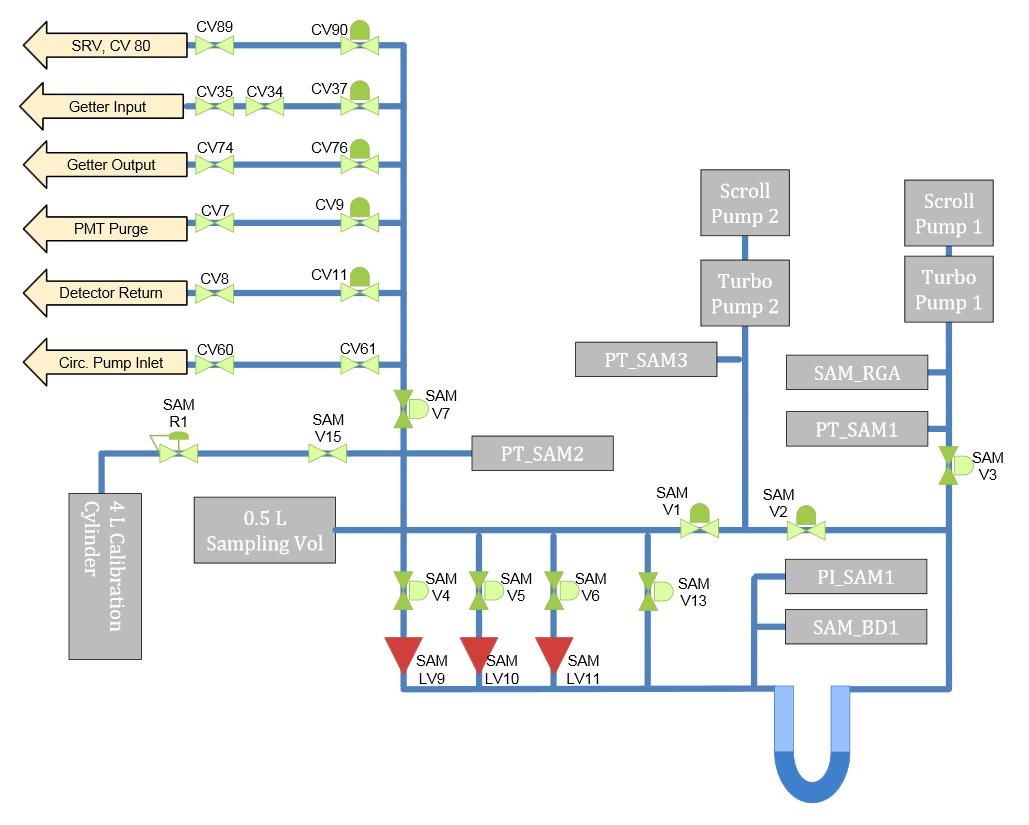
\includegraphics[scale=.3]{SAMdiagram.png} 
\captionof{figure}{Depiction of the LUX sampling system.  Xenon enters the sampling system through various sampling ports in the main circulation path. These sampling ports are shown in the top left of the diagram.  The xenon then passes through one of three leak valves (indicated by red triangles) into a U-shaped cold trap, where it is analyzed by an RGA on the output of the cold trap.  A secondary set of vacuum pumps is included so that the system can be evacuated independently of the RGA space.}
\label{LuxSamSystem}
\end{figure}


\subsubsection{Water Tank and Muon Veto System}

The LUX cryostat is enclosed in a 7.6 meter diameter, 5.1 meter high water tank.  The water tank holds 8 tons of water that is continuously circulated through an industrial purifying system to reduce detector backgrounds originating from the water tank itself.  The concentration of uranium, thorium, and potassium are held more than six orders of magnitude lower than the rock surrounding the laboratory (2 ppt, 3ppt, and 4 ppb respectively). The water tank provides 2.75 m of shielding to the top of the detector, and 3.5 m of shielding to the sides, that reduces backgrounds originating in the laboratory environment.  The tank is also outfitted with 20 Hammamatsu R7081 PMTs which can be used as an active veto for events which coincide with muons passing through the detector.

 \begin{figure} [!h]
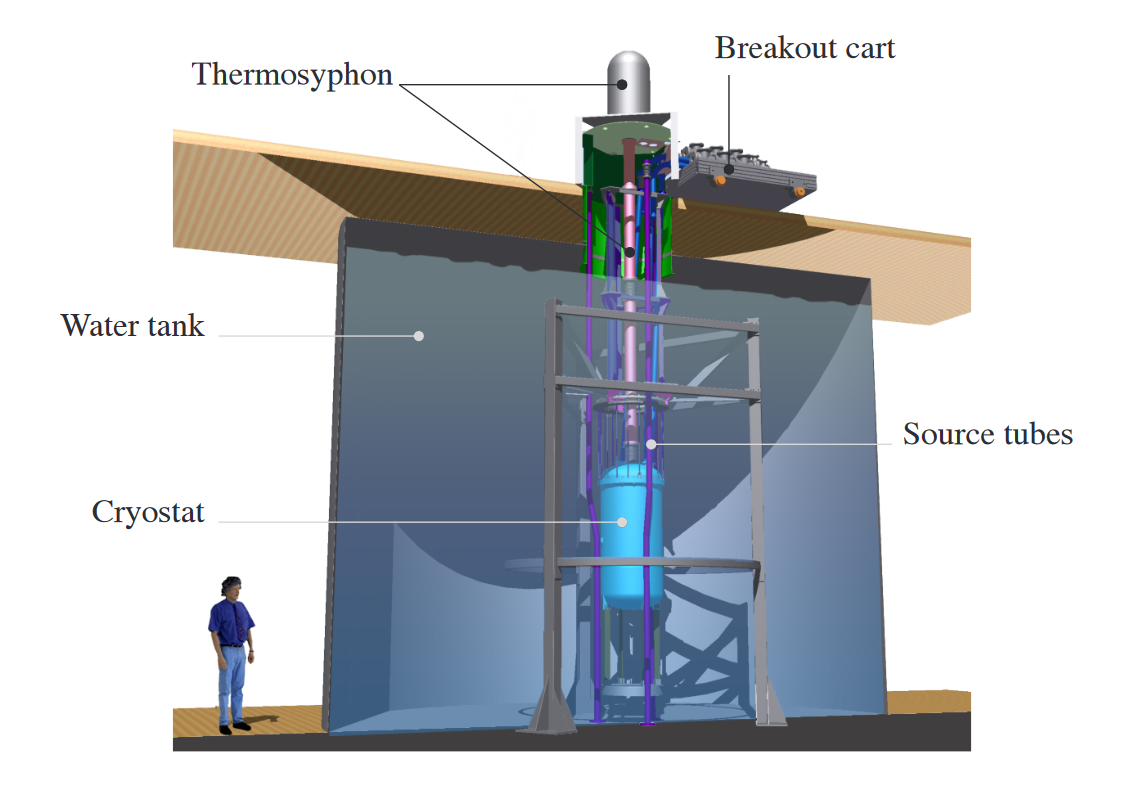
\includegraphics[scale=.35]{LuxWaterTank.png} 
\captionof{figure}{Cross section of the LUX water tank which surrounds the cryostat.}
\label{LuxWaterTank}
\end{figure}

\subsubsection{Calibration Systems}

LUX utilizes multiple internal and external calibration sources to measure the detector's S1 and S2 response to recoil events.  Six source tubes surround the cryostat in the water tank.  A system of pulleys allows radioactive sources to be deployed and retracted in each tube.  A collimator is used for directional control of the particle interactions from the external sources. AmBe and $^{252}$Cf neutron sources are placed in the source tubes to calibrate the detectors nuclear recoil response.  High energy $^{137}$Cs gamma ray sources are placed in the tubes to calibrate the detector's electron recoil response, and to illuminate the detector walls for position reconstruction and background modeling studies.  Other gamma ray sources, such as $^{22}$Na and $^{208}$Tl are available for electron recoil response calibration as well.  High energy gamma rays from external sources only penetrate the outermost centimeters of the liquid xenon volume due the same self shielding properties that reduce unwanted external backgrounds, making it difficult to calibrate the entire fiducial volume with external sources.

\begin{figure} [!h]
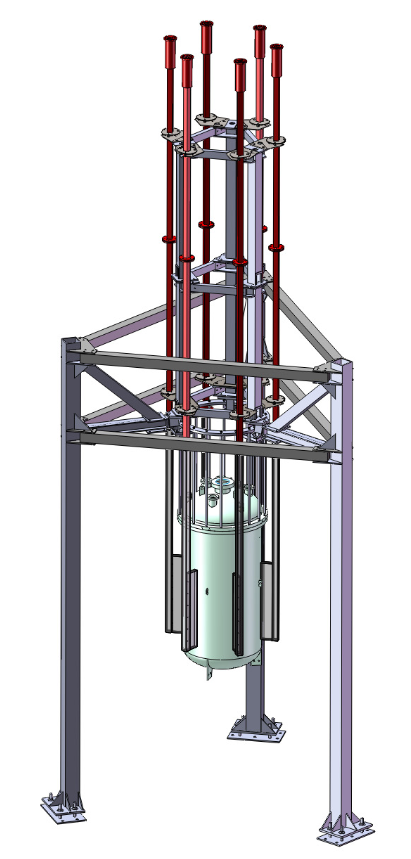
\includegraphics[scale=.35]{LuxSourceTubes.png} 
\captionof{figure}{Rendering of the six external source tubes which surround the LUX cryostat.}
\label{LuxSourceTubes}
\end{figure}

In addition to the source tubes mentioned above, a 377 cm long horizontal nitrogen filled conduit can be raised in the water tank by a pulley system.   This conduit serves to displace water from the tank, opening a collimation path for an external neutron beam.  The neutron generator is operated at a 5\% duty cycle using 100 $\mu$s neutron pulses to produce mono-energetic 2.45 MeV neutrons at a rate of 500 Hz. The resulting neutrons scatter multiple times in the fiducial volume, and are used to calibrate the detector's nuclear recoil response from 0.7 to 24.2 keV$_{nr}$.


LUX also employs two internal calibrations sources which are injected directly into the gas circulation system.   $^{83}$Rb soaked charcoal is used to inject $^{83m}$Kr directly into the circulation system on a weekly basis.  $^{83}$Rb decays into $^{83m}$Kr with an 86.2 day half life.   The resulting $^{83m}$Kr daughter decays via two sequential internal conversion electrons at 9.4 keV and 32.1 keV with a half life of 1.86 hours.  Once injected into the gas system, the $^{83m}$Kr quickly makes its way into the fiducial volume, where it uniformly disperses throughout the entire detector.  The spatial uniformity and intrinsic nature of this source makes it extremely useful when measuring the spatial dependence of the detector's S1 and S2 signals, which we will discuss in depth in Chapter~\ref{StandardCalibrations}.  After a calibration has finished, the $^{83m}$Kr is removed from the detector in a short amount of time due to its 1.86 hour half life.  

Tritiated methane (CH$_3$T) is the second internal calibration source used in LUX.  CH$_3$T is a beta source with a peak at 2.5 keV and a mean energy of 5.6 keV.  The wide, low energy spectrum of CH$_3$T is used to calibrate the detector's electron recoil response across the entire energy range of interest for WIMP events.  CH$_3$T has a half life of 12.3 years, so unlike the  $^{83m}$Kr it must be actively removed from the detector by the SAES getter in the circulation system.  The unprecedented CH$_3$T source was designed specifically for LUX, and is discussed in detail in Chapter~\ref{TritiumChapter}.


%From: http://xxx.lanl.gov/pdf/1108.1836v2
\subsection{Detector Electronics}

The photons collected by the two PMT arrays are amplified by the PMT dynode chains to mV scale voltage signals.  The rise time for an S1 pulse is limited to $\sim$6 ns by the response of the PMTs, and the 29 ns effective time constant of the xenon excimer relaxation defines the S1 pulses' decay constant.  The pulse width of an S2 event varies with depth due to diffusion of the electron cloud as it drifts through the detector. 

The LUX data acquisition (DAQ) system  is designed to distinguish $>$95\% of single photoelectron pulses at 5 sigma above baseline noise fluctuations, and to prevent saturation of events with energies $<$100 keV$_{ee}$ at any stage in the electronics.  To achieve this, the analog chain must put the peak of single photoelectron distribution at 30 ADC counts.  In the analog chain, the mV scale signals from the PMTs are sent to a x5 amplitude preamplifier before passing to a post amplifier in the DAQ electronics rack. The multichannel post amplifier produces a gain of 1.5x that is sent to sixteen 8-channel ADC modules, and a gain of 2.8x to a DDC-8 trigger system.

The ADC modules digitize the signals at 100 MHz (10 ns/sample) with a resolution of 14 bits. Each ADC board is connected to a VME bus that is subsequently connected to the DAQ computer by fiber optic cables.  Data is downloaded to the DAQ computer with speeds of up to 80 MB/s.  Each ADC board is controlled by four field programmable gate arrays (FPGAs) that operate in a space saving "pulse only digitization" (POD) mode. In POD mode, PMT channels are paired and data is only saved to the DAQ computer if either member of the PMT pairing rises above threshold. A valid pulse trigger gate (VPTG) mechanism further reduces memory space demands.  The VPTG is implemented using CAEN V814 discriminators which require two fold coincidence between PMT channels. Valid pulses are expected to occur in more than one channel, so the VPTG reduces unwanted triggers from various sources of noise.

The DAQ trigger system uses two 8 channel digital signal processors (DDC-8DSP).  
Top and bottom PMTs are summed into 16 groups (8 groups per array), and the analog sum of each group is produced with a Lecroy 628 Linear Fan-In/Fan-Out module.  
A trigger builder is connected to the DDC-8’s and takes $<$1 $\mu$second to generate a final trigger signal to send to the DAQ.  The trigger builder is capable of distinguishing S1 and S2 pulses, and can therefore operate in S1-only, S2-only, or S1 and S2 trigger mode.  The DAQ can operate with a maximum trigger rate of 1.5 kHz before incurring deadtime. 

\subsection{Science Results}

PUT RUN04 RESULT IF (OR RUN03 IF RUN04 ISNT AVAILABLE)

